\hypertarget{uxe9nergie-de-loscillateur-harmonique}{%
\section[Énergie de l'oscillateur
harmonique]{\texorpdfstring{\protect\hypertarget{anchor}{}{}Énergie de
l'oscillateur
harmonique}{Énergie de l'oscillateur harmonique}}\label{uxe9nergie-de-loscillateur-harmonique}}

\hypertarget{viduxe9os-uxe0-regarder-sur-youtube}{%
\subsection[Vidéos à regarder sur
YouTube]{\texorpdfstring{\protect\hypertarget{anchor-1}{}{}Vidéos à
regarder sur
YouTube}{Vidéos à regarder sur YouTube}}\label{viduxe9os-uxe0-regarder-sur-youtube}}

\begin{enumerate}
\def\labelenumi{\arabic{enumi}.}
\tightlist
\item
  \href{https://youtu.be/sXIMn32DK7A}{\emph{https://youtu.be/sXIMn32DK7A}}
\item
  \href{https://youtu.be/NrSj516RLQM}{\emph{https://youtu.be/NrSj516RLQM}}
\end{enumerate}

\hypertarget{diffuxe9rentes-formes-duxe9nergie-dun-oscillateur-harmonique}{%
\subsection[Différentes formes d'énergie d'un oscillateur
harmonique]{\texorpdfstring{\protect\hypertarget{anchor-2}{}{}Différentes
formes d'énergie d'un oscillateur
harmonique}{Différentes formes d'énergie d'un oscillateur harmonique}}\label{diffuxe9rentes-formes-duxe9nergie-dun-oscillateur-harmonique}}

\begin{enumerate}
\def\labelenumi{\arabic{enumi}.}
\tightlist
\item
  Energie cinétique~(due à la vitesse) : \[{E = \frac{1}{2}}mv^{2}\]
\item
  Energie potentielle gravifique (due à la hauteur)~:
  \[E = \mathit{mgh}\]
\item
  Energie potentielle élastique due à la compression ou dilatation d'un
  ressort)\[{E = \frac{1}{2}}ky^{2}\]
\end{enumerate}

\hypertarget{energie-totale-dun-oscillateur-harmonique}{%
\subsection[Energie totale d'un oscillateur
harmonique]{\texorpdfstring{\protect\hypertarget{anchor-3}{}{}Energie
totale d'un oscillateur
harmonique}{Energie totale d'un oscillateur harmonique}}\label{energie-totale-dun-oscillateur-harmonique}}

L'énergie totale mécanique d'un oscillateur harmonique est la somme des
énergies cinétique et potentielle (gravifique pour un pendule simple et
élastique pour un ressort horizontal).

Dans le cas où les frottements sont négligés, l'énergie totale reste
constante (principe de conservation d'énergie).

Exprimons mathématiquement ce principe en répondant à la question~:

En toute généralité, quelle est l'énergie totale d'un oscillateur
harmonique~ (que ce soit un pendule simple ou un pendule élastique)~?

Lorsqu'un oscillateur harmonique est à une position extrême (+A ou -A),
l'énergie cinétique est nulle et l'énergie potentielle maximale (énergie
potentielle gravifique pour un pendule simple et énergie potentielle
élastique pour un ressort horizontal).

De même, pour un oscillateur harmonique (quel qu'il soit), lorsque la
vitesse est maximale, l'énergie potentielle est nulle (énergie
potentielle gravifique pour un pendule simple et énergie potentielle
élastique pour un ressort horizontal). L'énergie totale de l'OH (ET) est
donc égale à\[{E = \frac{1}{2}}mv_{\text{max}}^{2}\]

Or nous savons que :
\[{E_{\text{totale}} = \frac{1}{2}}mv_{\text{max}}^{2}\] avec
\[{v_{\text{max}} = A}\omega\]. Donc
\[{E_{\text{totale}} = \frac{1}{2}}m{v_{\text{max}}^{2} = \frac{1}{2}}mA^{2}\omega^{2}\]

Or \[T\] et \[\omega\] ne varient pas au cours de l'oscillation, elles
sont constantes.

Notons\[{k = m}\omega^{2}\] où k est une constante. On
trouve\[{E_{\text{totale}} = \frac{1}{2}}kA^{2}\]

qui est donc l'énergie totale d'un oscillateur harmonique.

\hypertarget{section}{%
\subsection{}\label{section}}

\hypertarget{que-repruxe9sente-k}{%
\subsection[Que représente k~?
]{\texorpdfstring{\protect\hypertarget{anchor-4}{}{}Que représente k~?
}{Que représente k~? }}\label{que-repruxe9sente-k}}

L'énergie totale d'un oscillateur harmonique
est~\[{E_{\text{totale}} = \frac{1}{2}}kA^{2}\]:

Que représente physiquement cette constante \[{k = m}\omega^{2}\]?

Pour un pendule élastique (un ressort)

k est la constante de raideur du ressort \[{F = k}x\](loi de Hooke) où
\[x\]~étant l'allongement du ressort à l'équilibre lorsque ce dernier
est soumis à une force de traction (ou de compression) F.

(Loi de Hooke)

Pour un pendule simple k =\[{k = m}\omega^{2}\]
\[{\omega = 2}\frac{\pi}{T}\]et
\[{T = 2}\pi\sqrt{\frac{L}{g}}\text{donc}{\omega^{2} = \frac{4\pi^{2}}{T^{2}} = {4\pi^{2}}}\frac{1}{4\pi^{2}}{\frac{g}{L} = \frac{g}{L}}\]

à où \[L\]~: longueur du pendule et \[m\]~: masse du pendule

\hypertarget{evolution-au-cours-du-temps-des-uxe9nergies-cinuxe9tique-potentielle-et-totale.}{%
\subsection[Evolution au cours du temps des énergies cinétique,
potentielle et totale.
]{\texorpdfstring{\protect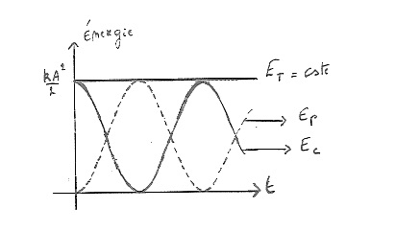
\includegraphics[width=8.183cm,height=4.821cm]{Pictures/100000010000018B000000E85C3B5046EC401703.png}\protect\hypertarget{anchor-5}{}{}Evolution
au cours du temps des énergies cinétique, potentielle et totale.
}{Evolution au cours du temps des énergies cinétique, potentielle et totale. }}\label{evolution-au-cours-du-temps-des-uxe9nergies-cinuxe9tique-potentielle-et-totale.}}

Variation de l'énergie cinétique
\[E_{c}{{(t)} = \frac{1}{2}}mv{{(t)} = \frac{1}{2}}m\omega^{2}A^{2}\text{cos}^{2}{({\omega{t + \phi}})}\]

Variation de l'énergie potentielle
\[E_{p}{{(t)} = \frac{1}{2}}{\mathit{ky}^{2} = \frac{1}{2}}kA^{2}\text{sin}^{2}{({\omega{t + \phi}})}\]

L'énergie totale reste constante. Elle est égale à la somme des énergies
cinétique et potentielle.

\[E_{c}{{(t)} + E_{p}}{{(t)} = E_{t} = \text{constante}}\]

\hypertarget{energie-dun-oscillateur-harmonique---exercices}{%
\subsection[Energie d'un oscillateur harmonique -
Exercices]{\texorpdfstring{\protect\hypertarget{anchor-6}{}{}Energie
d'un oscillateur harmonique -
Exercices}{Energie d'un oscillateur harmonique - Exercices}}\label{energie-dun-oscillateur-harmonique---exercices}}

\begin{figure}
\centering
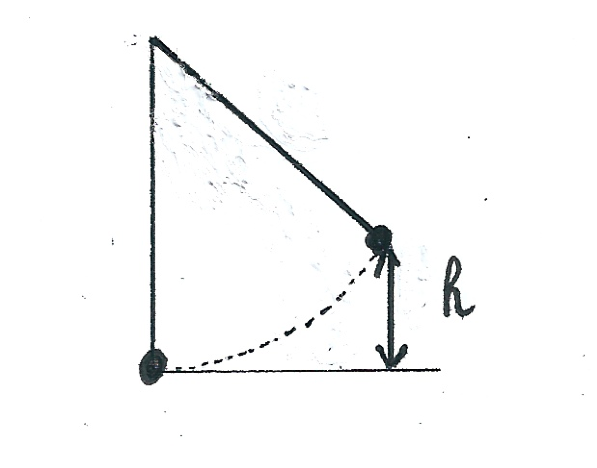
\includegraphics[width=5.457cm,height=4.239cm]{Pictures/1000000100000255000001D4999CDF6CC98F91D9.png}
\caption{}
\end{figure}

\hypertarget{exercice-1}{%
\subsubsection[Exercice
1]{\texorpdfstring{\protect\hypertarget{anchor-7}{}{}Exercice
1}{Exercice 1}}\label{exercice-1}}

Un pendule simple de longueur égale à 40 cm et d'une masse de 50 g est
lâché lorsqu'il fait un angle de 10° avec la verticale.

\begin{enumerate}
\def\labelenumi{\arabic{enumi}.}
\tightlist
\item
  Calculez son énergie potentielle maximale.
\item
  Calculez sa vitesse maximale.
\item
  Calculez sa vitesse à mi-hauteur.
\item
  Quelle est son énergie totale~?
\end{enumerate}

\hypertarget{exercice-2}{%
\subsubsection[Exercice
2]{\texorpdfstring{\protect\hypertarget{anchor-8}{}{}Exercice
2\protect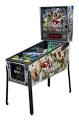
\includegraphics[width=2.688cm,height=4.12cm]{Pictures/100000000000004F00000079BF194595D71050C5.png}}{Exercice 2}}\label{exercice-2}}

Pour lancer une boule (masse 50 g) de « flipper », on comprime de 10 cm
un ressort d'une constante de raideur égale à 200 N/m. Quelle sera la
vitesse de la boule lorsqu'elle aborde le virage au bout d'une course
rectiligne de 1,5 m après qu'elle ait quitté le ressort. Négligez tout
frottement !

\begin{enumerate}
\def\labelenumi{\arabic{enumi}.}
\tightlist
\item
  si le flipper est horizontal ?
\item
  s'il fait un angle de 5° avec l'horizontale ?
\end{enumerate}

\hypertarget{exercice-3}{%
\subsubsection[Exercice
3]{\texorpdfstring{\protect\hypertarget{anchor-9}{}{}\protect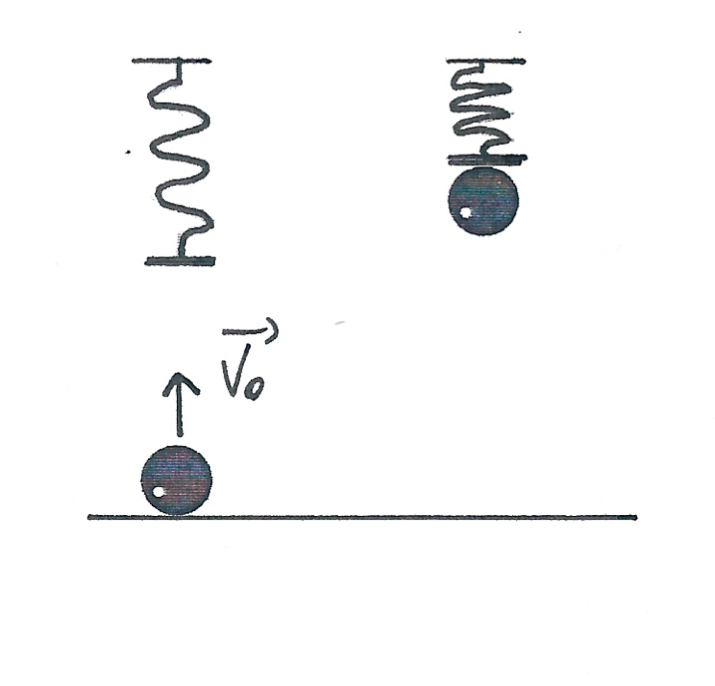
\includegraphics[width=5.75cm,height=5.539cm]{Pictures/10000001000002CB000002AEBE5814C250A43575.png}Exercice
3}{Exercice 3}}\label{exercice-3}}

Une balle de 500g est lancée verticalement vers le haut sur un ressort
de constante de raideur égale à 32 N/m et de masse négligeable. La
vitesse de lancer de 2 m/s.

Le ressort se comprime de 12 cm lorsque la bille atteint sa hauteur
maximale.

Quelle est la hauteur atteinte par la bille~?

\hypertarget{exercice-4}{%
\subsubsection[Exercice
4]{\texorpdfstring{\protect\hypertarget{anchor-10}{}{}Exercice
4}{Exercice 4}}\label{exercice-4}}

Un fusil de fléchettes comprend un ressort de raideur k = 250 N/m, de
longueur à vide l0 = 12 cm et qui, comprimé par la fléchette de masse 25
g, ne mesure plus que l = 4,0 cm.

\begin{enumerate}
\def\labelenumi{\arabic{enumi}.}
\item
  Avec quelle vitesse la fléchette sort-elle du fusil dans le cas d'un
  tir horizontal. Faire le calcul sans tenir compte du frottement entre
  fléchette et fusil.
\item
  Quelle altitude maximale peut-elle atteindre dans le cas d'un tir
  vertical ? Faire le calcul sans tenir compte du frottement entre
  fléchette et fusil ni de la résistance de l'air.
\end{enumerate}

\hypertarget{exercice-5}{%
\subsubsection[Exercice
5]{\texorpdfstring{\protect\hypertarget{anchor-11}{}{}Exercice
5\protect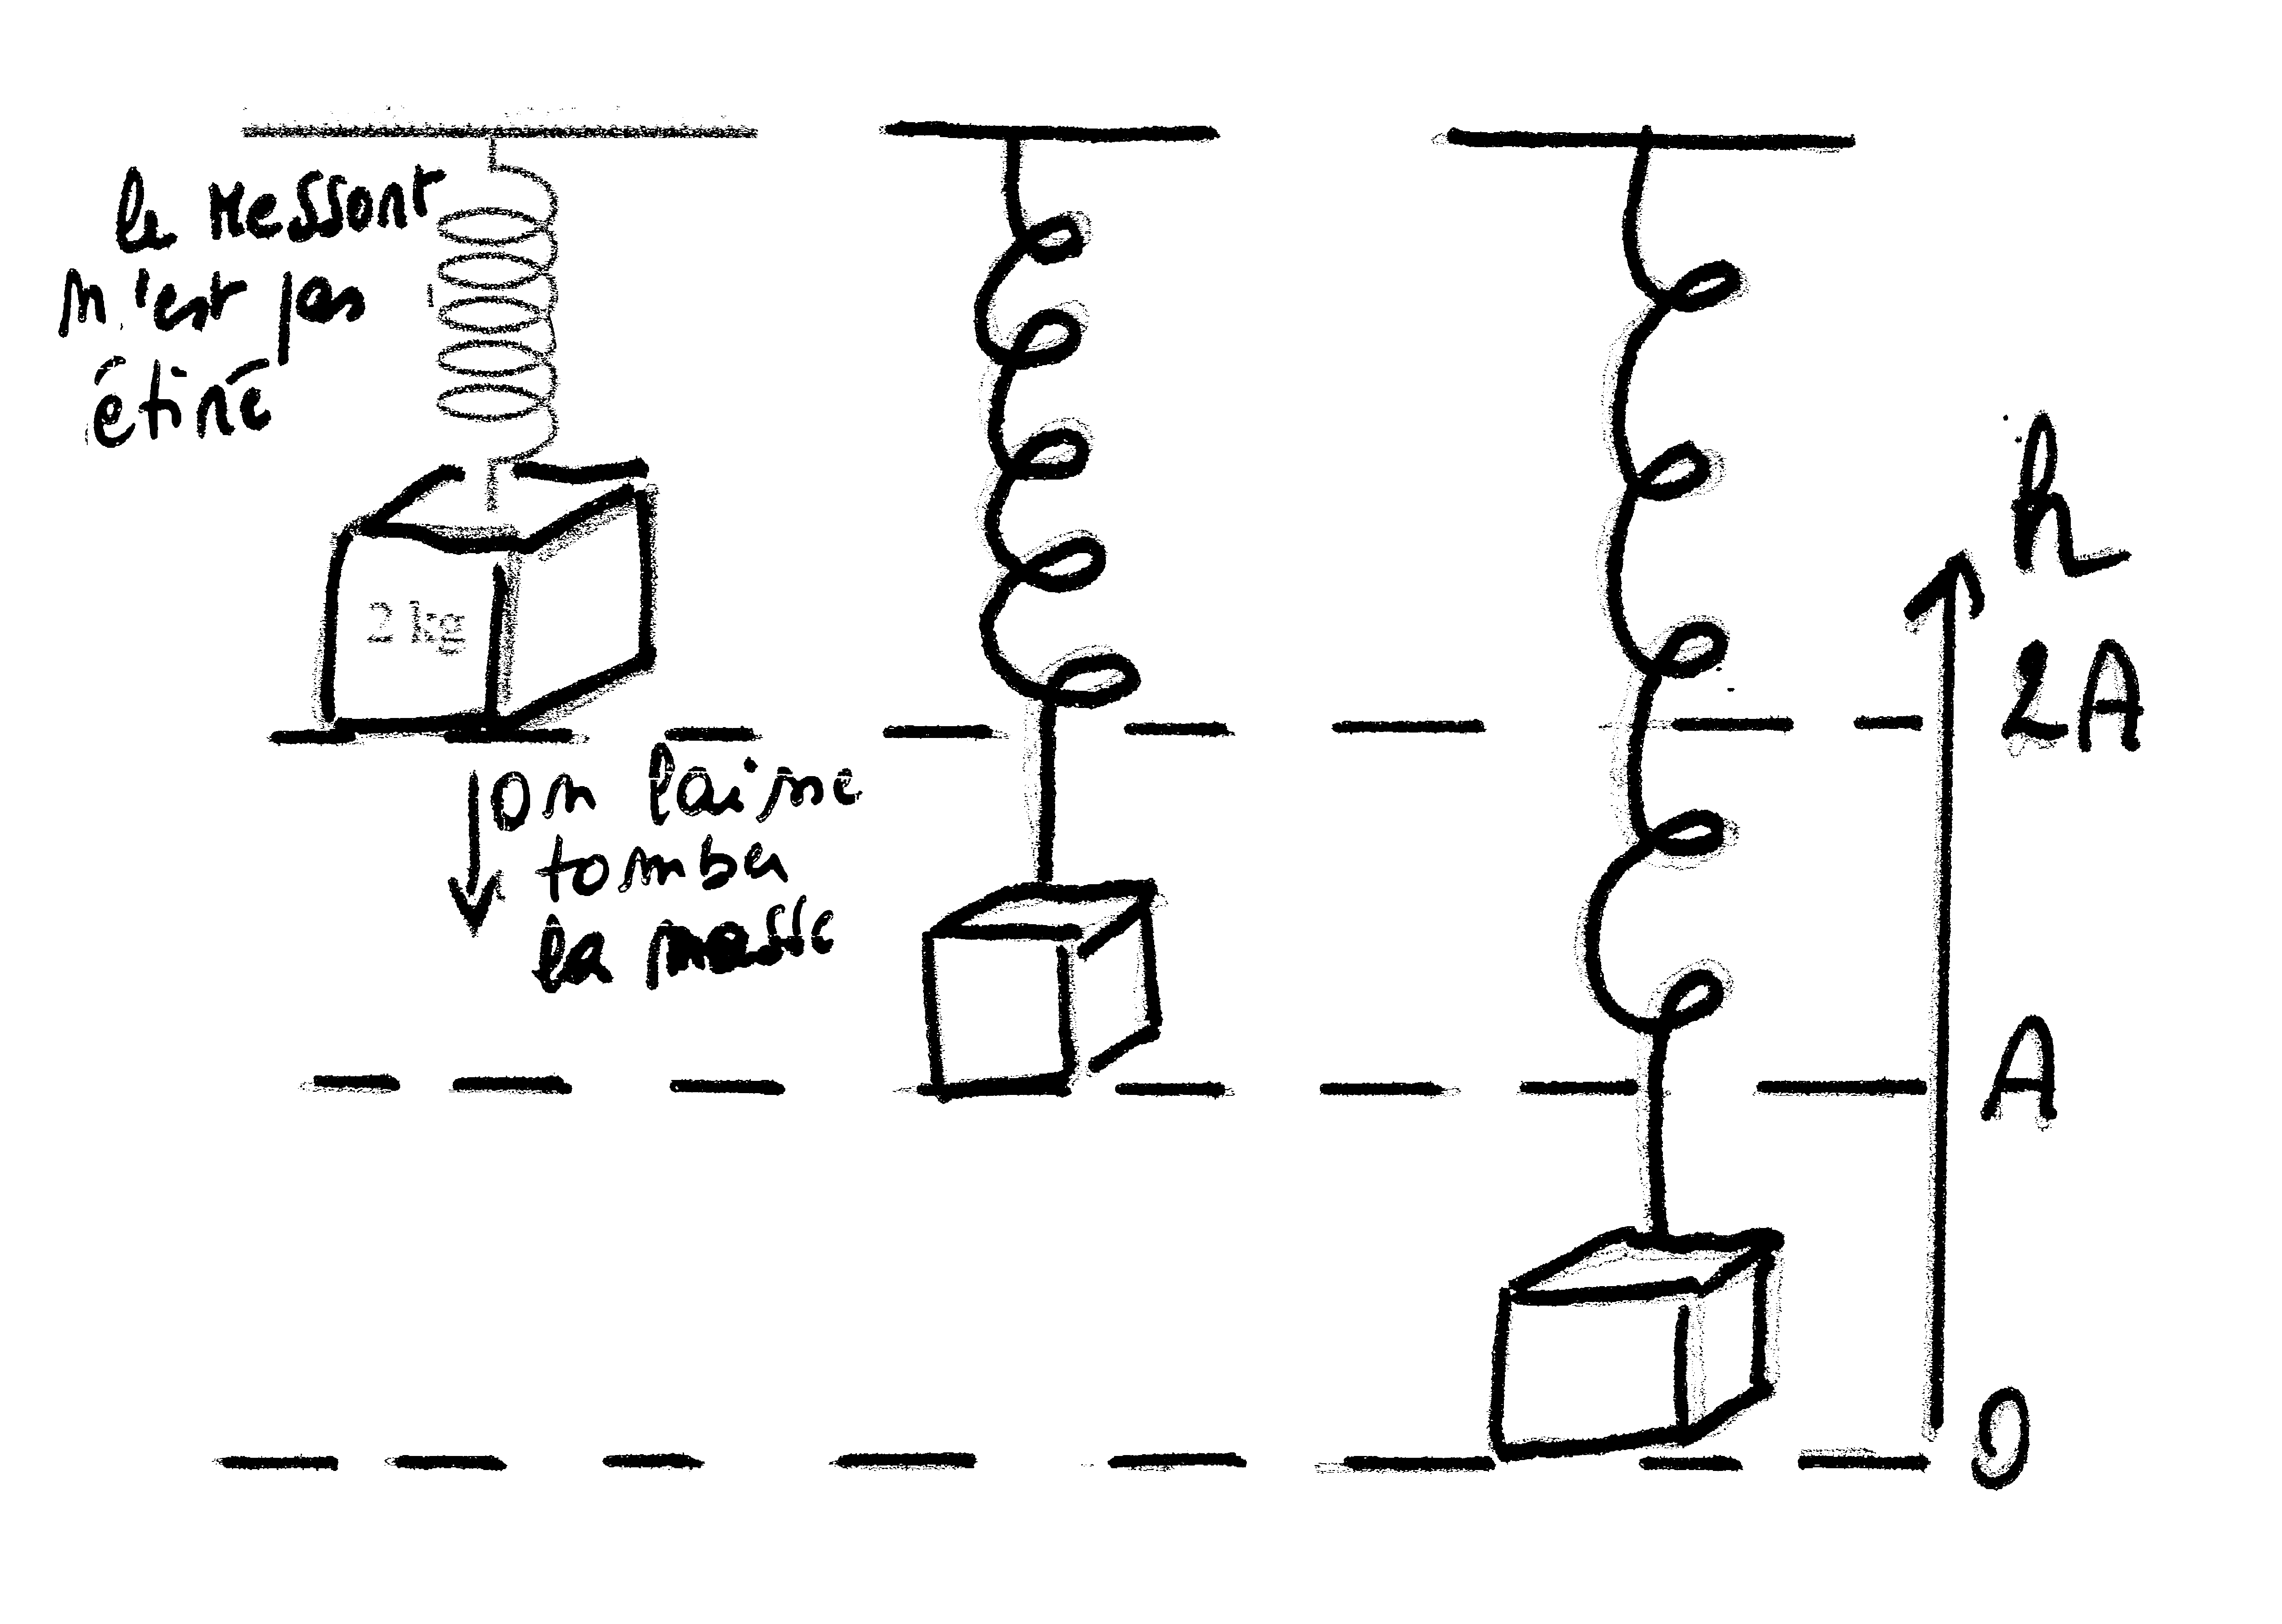
\includegraphics[width=8.373cm,height=5.95cm]{Pictures/10000000000013A000000DF82AB24E2F70D0A5A2.png}}{Exercice 5}}\label{exercice-5}}

La masse de 2 kg de la figure ci-contre est suspendue au plafond avec un
ressort de masse négligeable et dont la constante de raideur vaut 200
N/m. Au départ, le ressort n'est pas étiré ni comprimé. On laisse alors
tomber la masse sans la pousser. On aura alors un mouvement
d'oscillation de la masse.

\begin{enumerate}
\def\labelenumi{\alph{enumi})}
\tightlist
\item
  Quelle sera la distance parcourue par le ressort avant qu'il n'entame
  sa remontée verticale~?
\item
  Quelle sera la vitesse maximale du ressort~?
\end{enumerate}

\begin{figure}
\centering
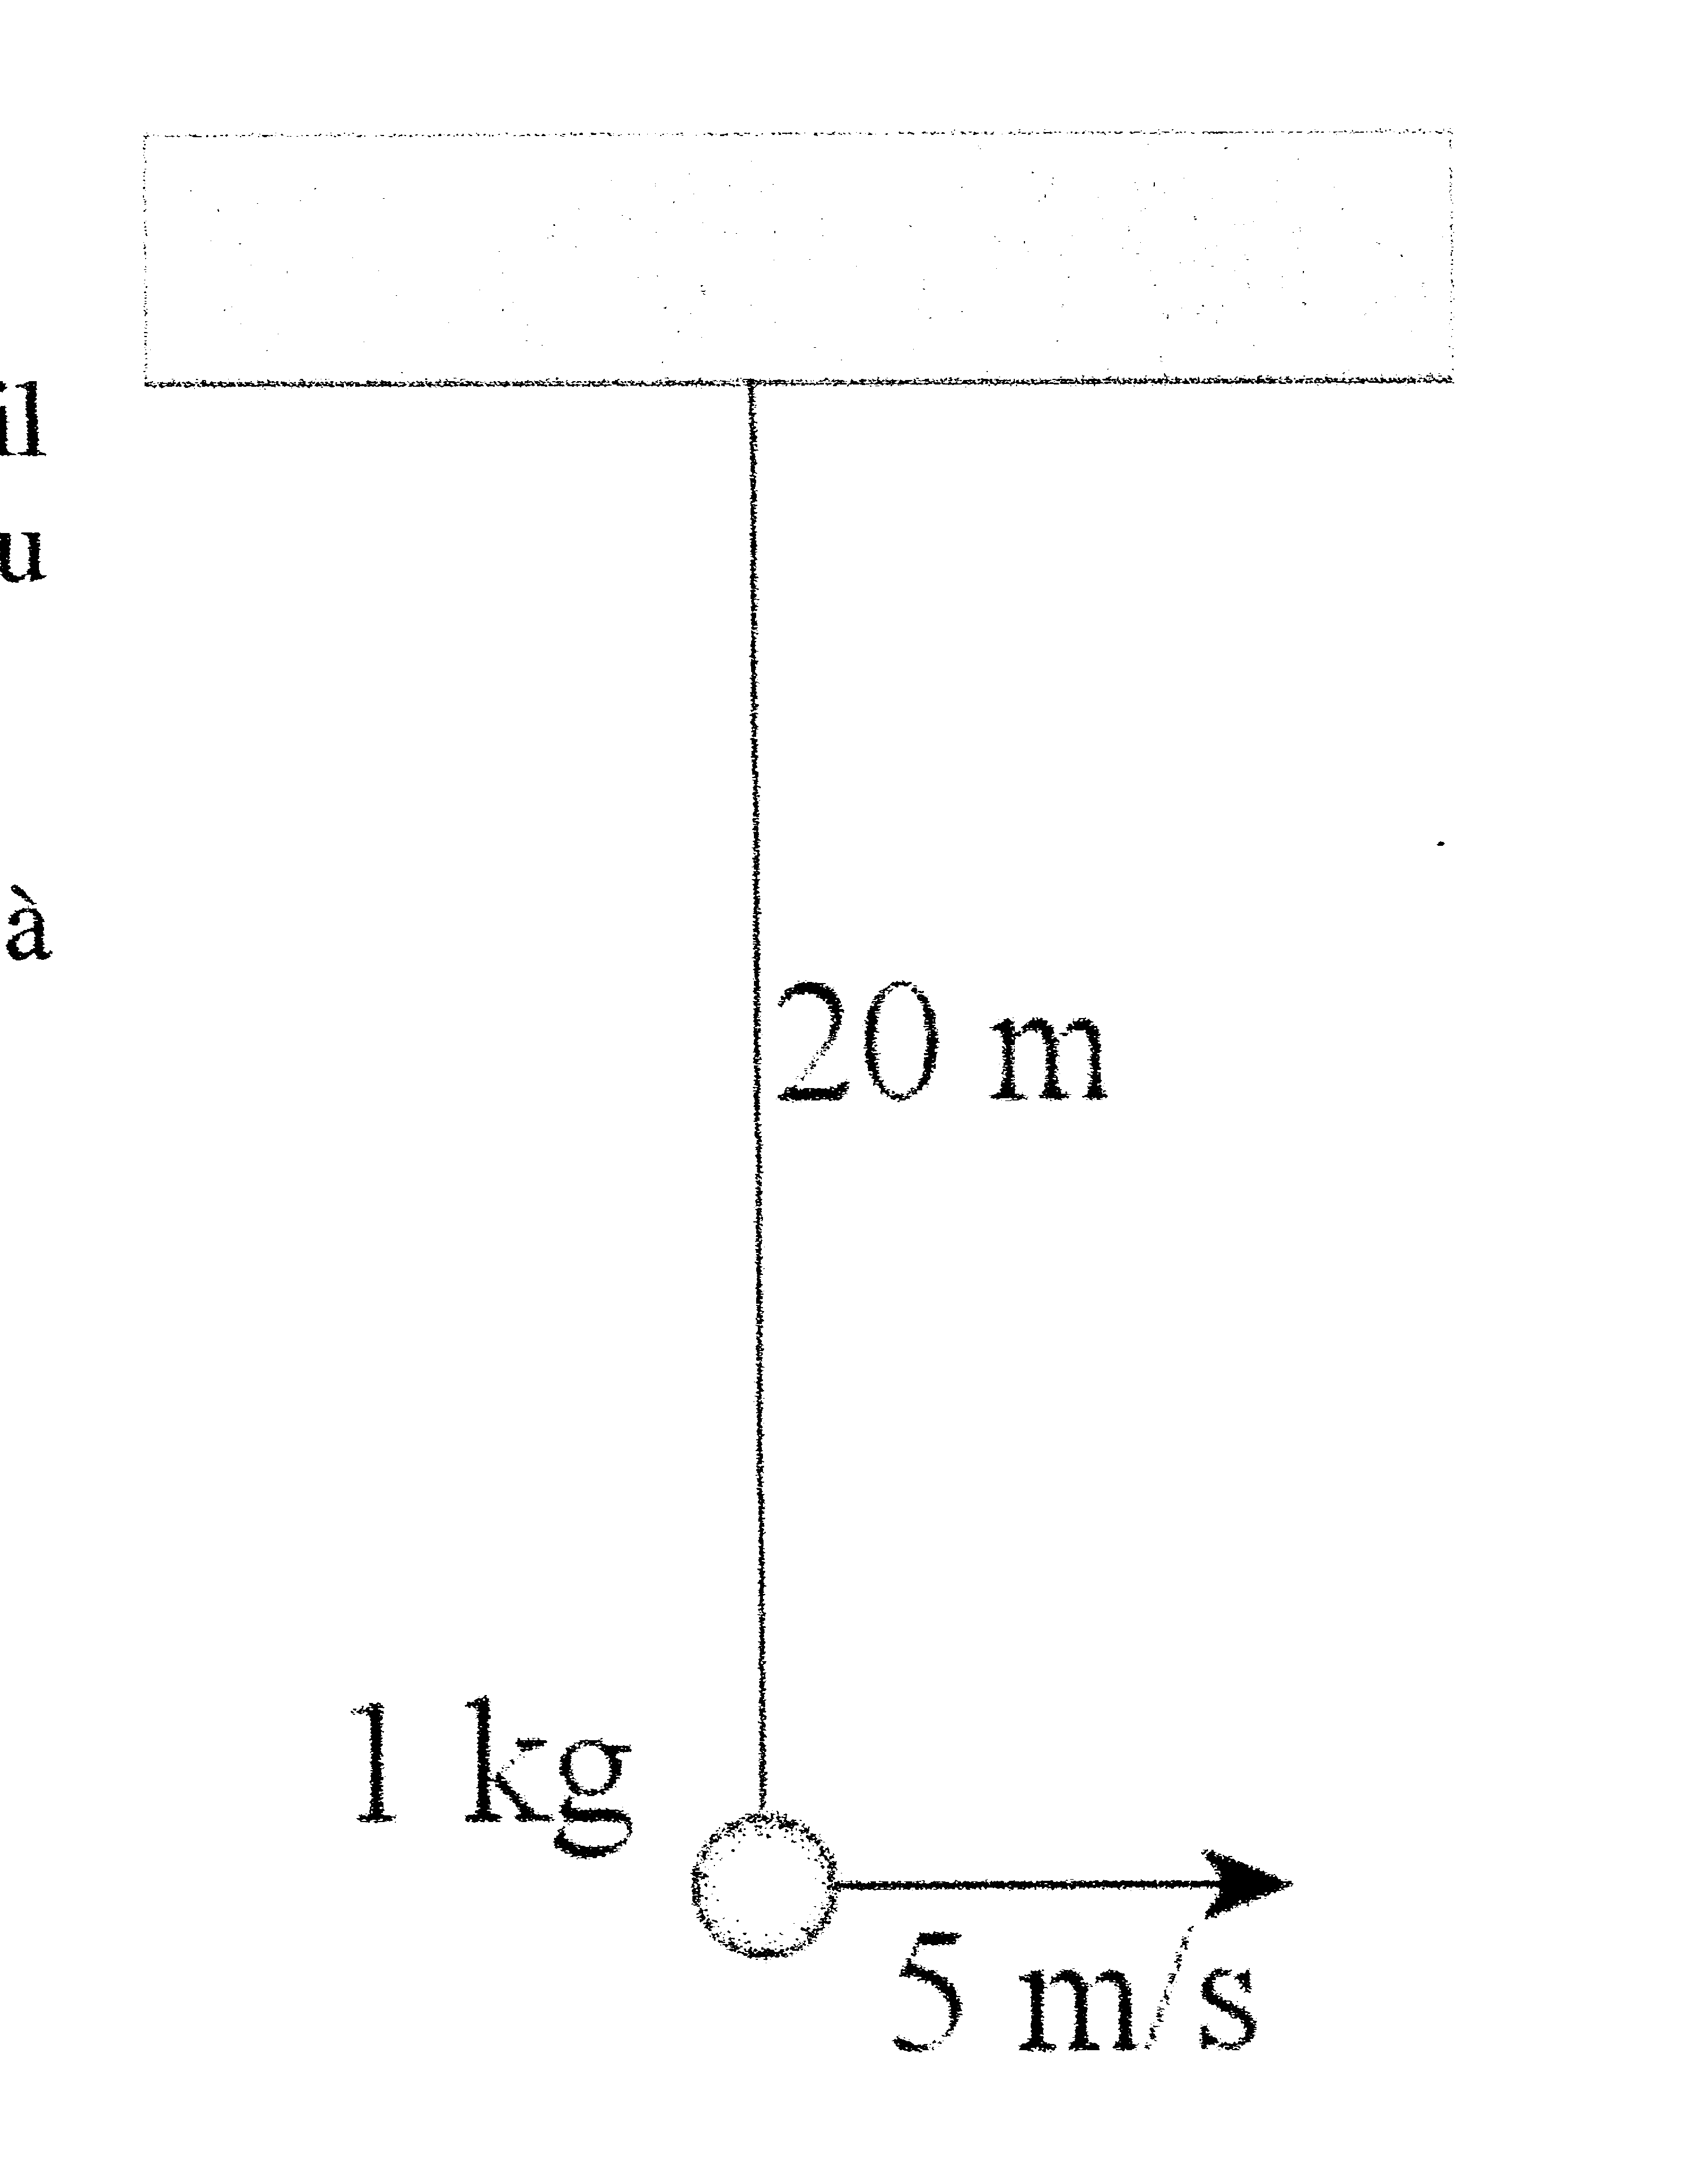
\includegraphics[width=3.17cm,height=4.47cm]{Pictures/1000000000000BC400000F1CA9B74E9E2E8AAFA4.png}
\caption{}
\end{figure}

\hypertarget{exercice-6}{%
\subsubsection[Exercice
6]{\texorpdfstring{\protect\hypertarget{anchor-12}{}{}Exercice
6}{Exercice 6}}\label{exercice-6}}

Le pendule de la figure ci-contre est en mouvement harmonique et a une
vitesse de 5 m/s quand il passe par sa position d'équilibre. Quelle est
la vitesse du pendule lorsqu'il fait un angle de 10° par rapport à la
verticale~?

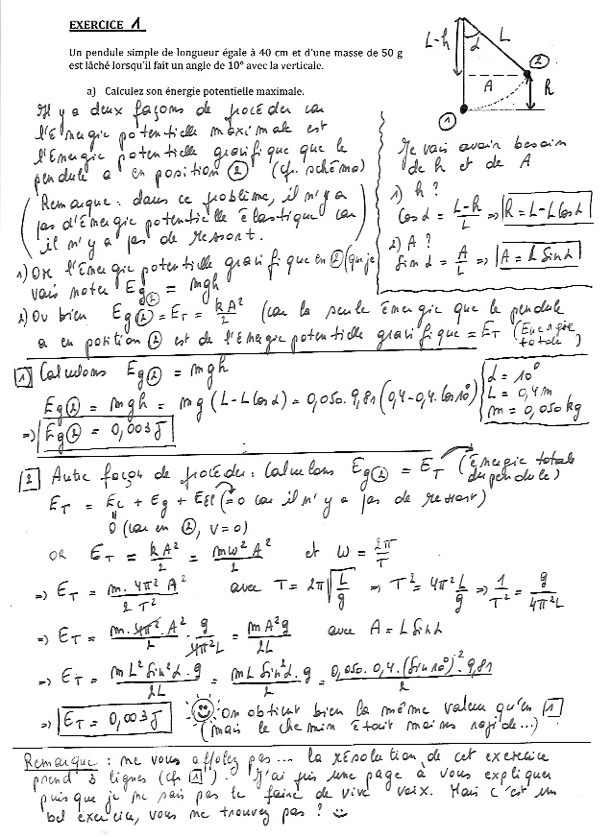
\includegraphics[width=17.498cm,height=26.033cm]{Pictures/1000000100000264000003450BBDC1031D5BD847.png}

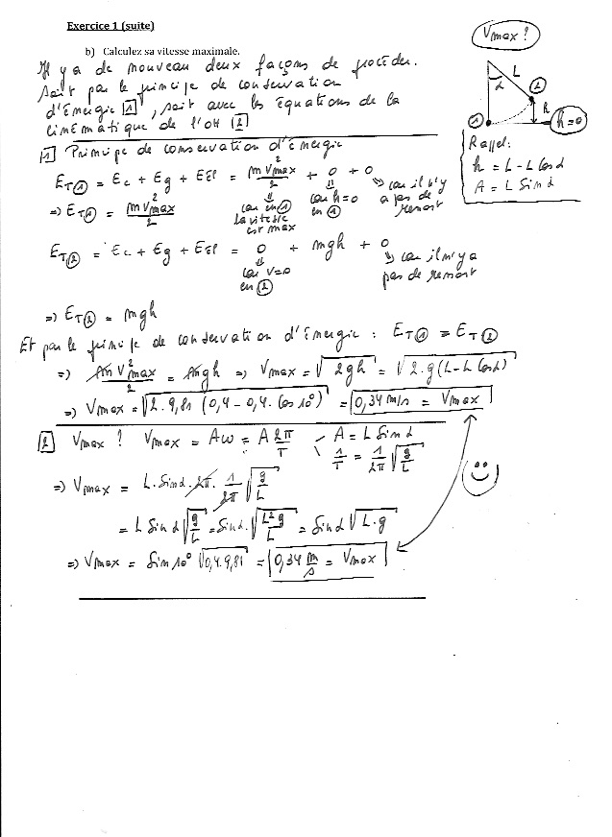
\includegraphics[width=17.498cm,height=26.174cm]{Pictures/1000000100000264000003457EC57F1EEB41A85F.png}

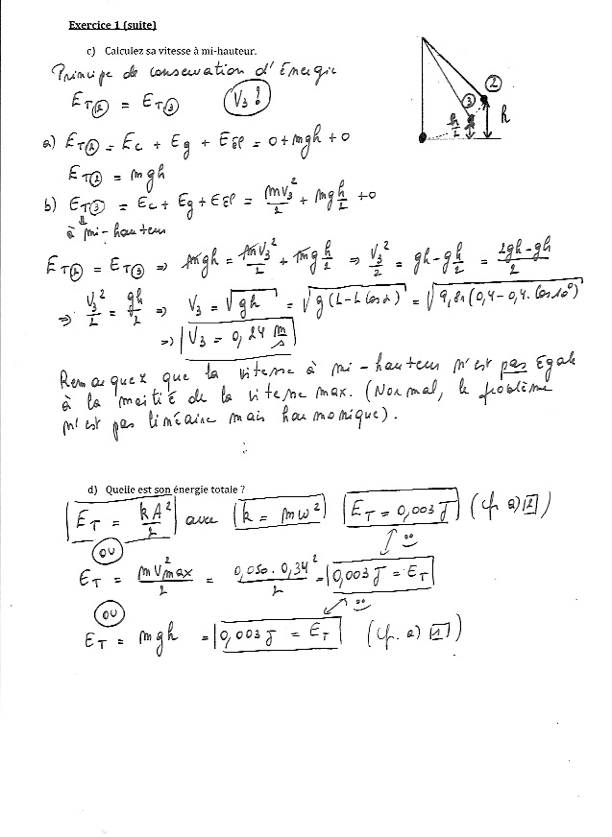
\includegraphics[width=17.498cm,height=23.941cm]{Pictures/1000000100000264000003450C3A378F8D932159.png}

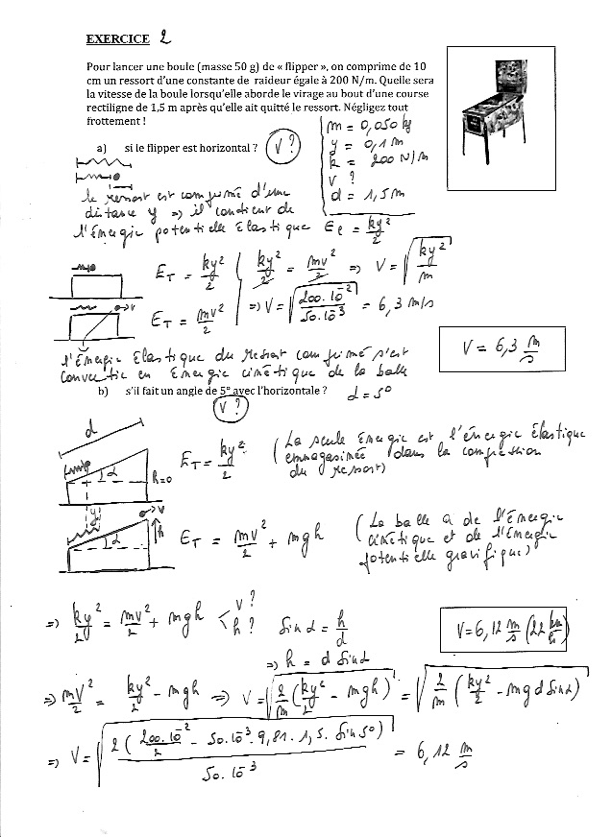
\includegraphics[width=17.498cm,height=24.552cm]{Pictures/100000010000026400000345AA0147C4E87FFA0E.png}

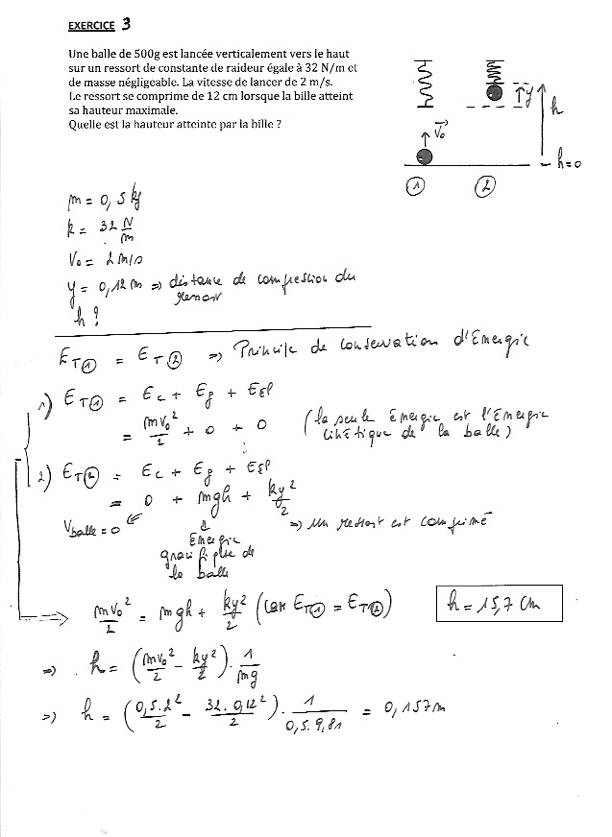
\includegraphics[width=17.498cm,height=23.941cm]{Pictures/1000000100000264000003455C9DE3ADDE2F2C0A.png}

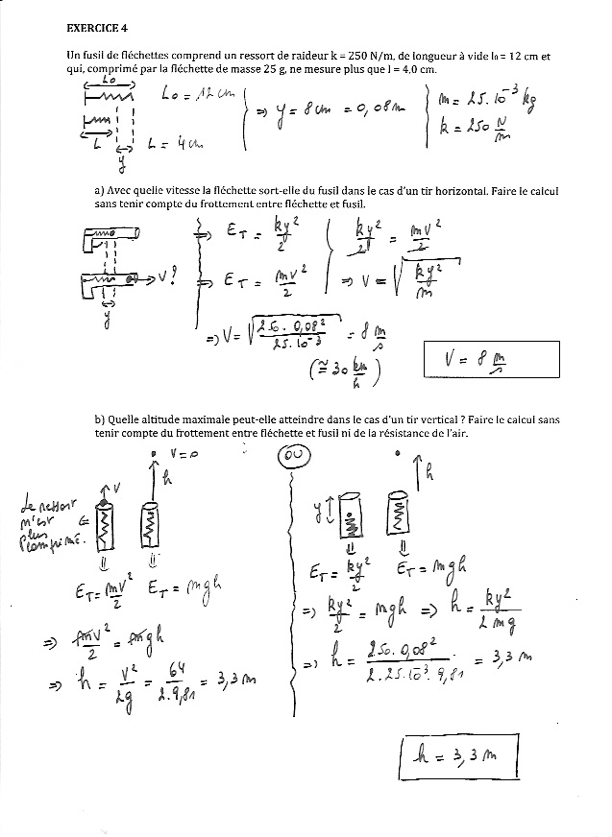
\includegraphics[width=17.498cm,height=23.941cm]{Pictures/100000010000026400000345A27521696B730F2D.png}

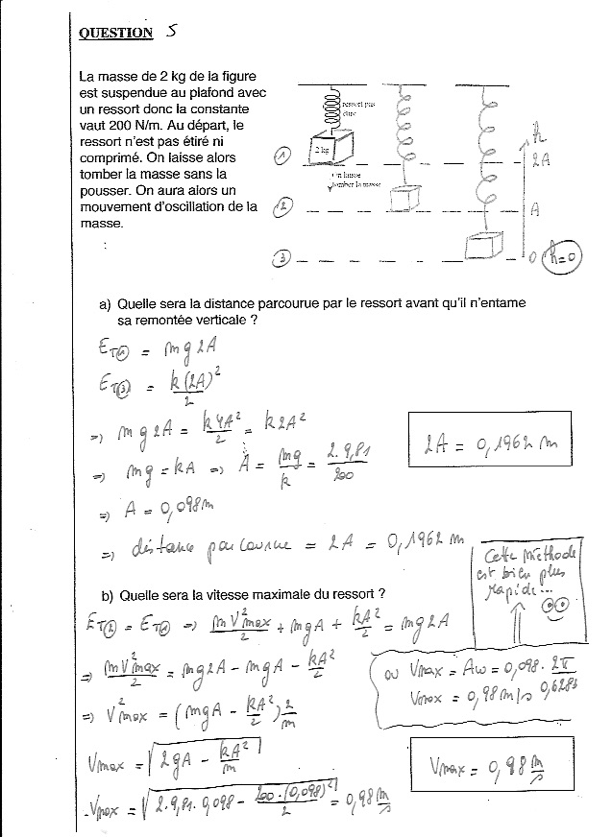
\includegraphics[width=18.196cm,height=24.897cm]{Pictures/100000010000026400000345B30134D27454F986.png}

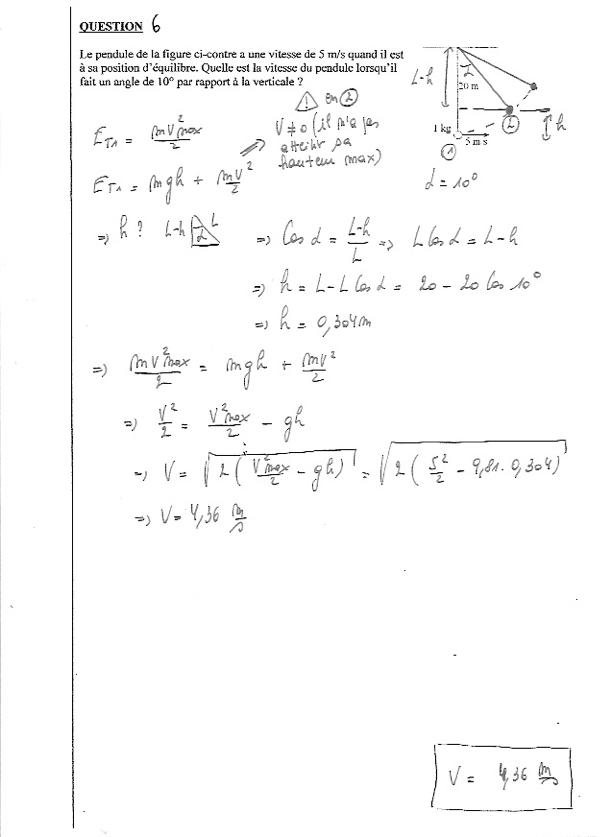
\includegraphics[width=17.498cm,height=23.941cm]{Pictures/100000010000026400000345CD11555FB30FBF68.png}
